\documentclass[tikz,border=6pt]{standalone}

\usepackage{siunitx}
\usepackage{xcolor}

% shared cartoon info
\usepackage{xcolor}
\usepackage{siunitx}
\usepackage{tikz}
\usetikzlibrary{calc,arrows.meta,backgrounds}

\newcommand{\Lx}{1}
\newcommand{\Ly}{3}
\newcommand{\Lz}{3}
\newcommand{\R}{0.25} % sphere radius = 1/3 (diameter 2/3)

\def\nuclei{
  0.15/0.60/0.70,
  0.35/1.40/2.50,
  0.75/2.10/1.10,
  0.60/0.90/2.20,
  0.20/2.60/0.50,
  0.90/1.80/1.70
}

\newcommand{\xcut}{0.05}

% Colors (example)
\definecolor{wcprimary}{RGB}{081,040,136}
\definecolor{wcalerted}{RGB}{202,124,027}
\definecolor{wcexample}{RGB}{000,134,086}

\tikzset{
  box/.style      = {line width=0.5pt, draw=black},
  nucleus3D/.style= {draw=black, fill=black!15},
  nucleus2D/.style= {draw=black, fill=black!25},
  beam/.style     = {-{Latex[length=2.2mm,width=1.8mm]},  thick},
  axislabel/.style= {font=\scriptsize},
  yzplane/.style = {fill=black,fill opacity=0.15},
  cutring/.style = {draw=black, dashed, line width=0.5pt, dash pattern=on 2pt off 1.2pt}
}




\begin{document}
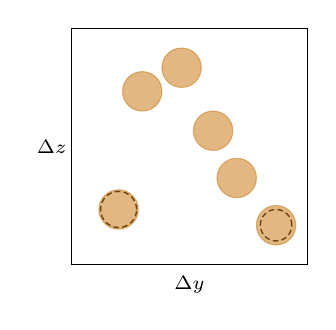
\begin{tikzpicture}[scale=1]
  % yz rectangle: width=Ly (y), height=Lz (z)
  % We'll draw inside a clip so circles are truncated by the slab outline.
  \begin{scope}
    \clip (0,0) rectangle (\Ly,\Lz);
    % Circles = intersection of each sphere with plane x = xcut
    % r_i = sqrt( R^2 - (x_i - xcut)^2 ), clipped at 0
    \foreach \x/\y/\z in \nuclei {
      \pgfmathsetmacro{\dx}{\x - \xcut}
      \pgfmathsetmacro{\rr}{sqrt(max(0, \R*\R - \dx*\dx))}
      \ifdim \rr pt>0pt
        \draw[cutring] (\y,\z) circle[radius=\rr cm];
      \fi
    }
    \foreach \x/\y/\z in \nuclei {
    \draw[nucleus2D, opacity=0.55, color=wcalerted] (\y,\z) circle[radius=\R cm];
    }
  \end{scope}
  % Frame and labels
  \draw[box] (0,0) rectangle (\Ly,\Lz);
  \node[axislabel] at (\Ly/2,-0.25) {$\Delta y$};
  \node[axislabel] at (-0.25,\Lz/2) {$\Delta z$};
\end{tikzpicture}
\end{document}
